\section{Uppgift 8}\label{sec:uppg08}

\subsection{Instruktioner}
\begin{verbatim}
8. Skriv en klass Person som innehåller följande instansvariabler, deklarera
   med passande datatyper:

        namn, personnummer, adress, ålder.

   I klassen ska följande metoder ingå:

   * konstruktorn Person, som initierar samtliga instansvariabler.
   * byterNamn, en metod som via parameter ändrar namnet.
   * byterAdress, en metod som via parameter ändrar adressen.
   * fyllerÅr, en metod som lägger till 1 till åldern.
   * hamtaNamn, en metod som returnerar namnet.
   * hamtaPersnr, en metod som returnerar personnumret.
   * hamtaÅlder, en metod som returnerar åldern.
   * hamtaAdress, en metod som returnerar adressen.
   * toString, en metod som i en snyggt formaterad sträng returnerar ett
     Person-objekts *samtliga* data.  Metoden anropas genom att skriva
     objektets (referensens) namn.

   Skriv ett testprogram som testar samtliga metoder i klassen Person.
   Programmet ska i tur och ordning utföra följande:

   * Skapa två Person-objekt, person1 och person2. Den som kör ditt program ska
     mata in startvärden till de båda objektens samtliga data
     (instansvariabler).
   * Skriv ut de båda objektens samtliga data.
   * Låt den som kör ditt program byta namn och adress på person1.
   * Låt person2 fylla år.
   * Skriv ut namnet, personnr och adressen på person1 (skriv alltså inte ut
     åldern).
   * Skriv ut namnet, personnr och åldern på person2 (skriv alltså inte ut
     adressen).
\end{verbatim}


\subsection{Lösning}
\subsubsection{Funktion}
% TODO: Eventuell beskrivning av #08 funktionalitet.

\subsubsection{Kommentar}
% TODO: Eventuell kommentar på #08.


\subsubsection{Källkod}
\javacode{src/main/Lab2Uppg08.java}
%\caption{Lab2Uppg08.java}
\label{src:uppg08}

\javacode{src/main/Person.java}
%\caption{Person.java}
\label{src:Person}


\subsubsection{Skärmdump}
\begin{figure}[htbp]
    \centering
        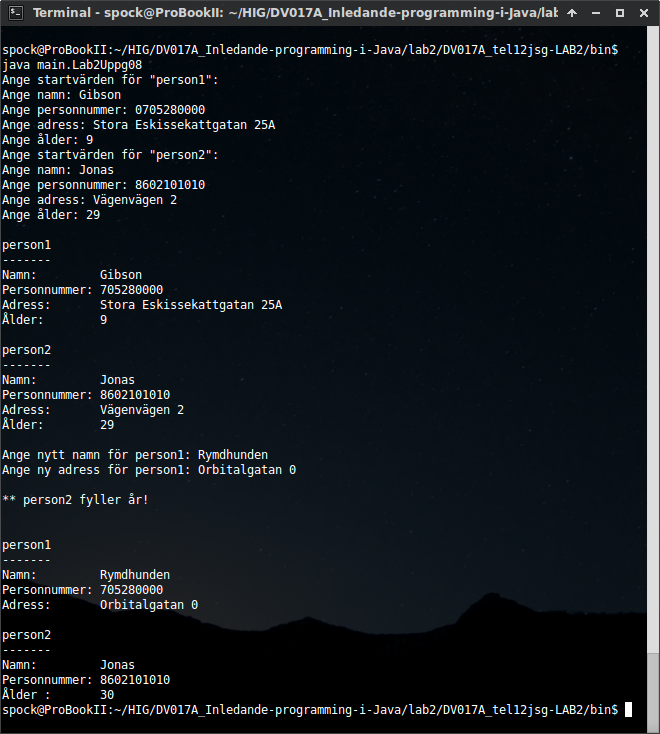
\includegraphics[width=\linewidth]{img/08.png}
    \caption{Körning av koden till Uppgift~\ref{sec:uppg08}}
    \label{fig:uppg08-screenshot}
\end{figure}
% TODO: Lägg till skärmdump av #08.

